\section{Introduction}

\begin{frame}{\secname}{3D world $\rightarrow$ 2D content}
    An image is just a flat representation of the 3D world.
    \begin{figure}
        \centering
        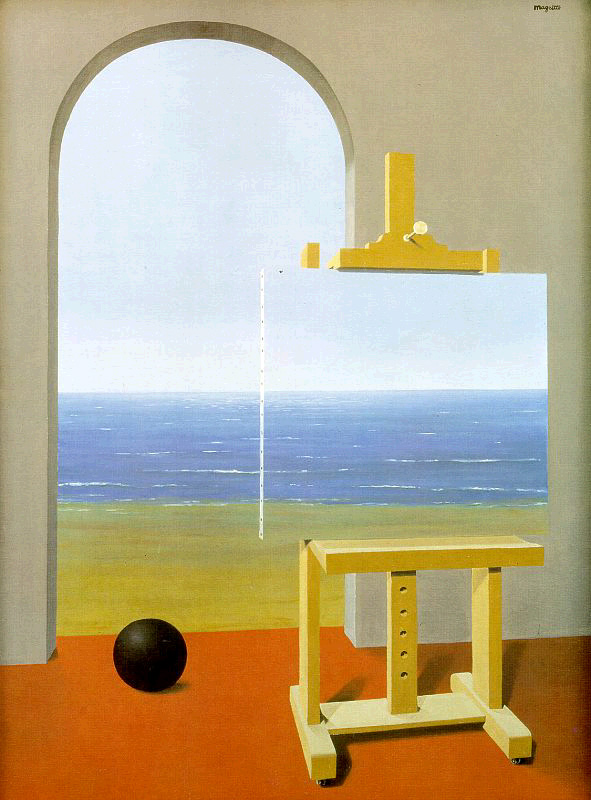
\includegraphics[height=0.5\textheight]{img/Magritte-human-condition.jpg}
    \end{figure}
    Even though we lose the depth component the image maintain the perspective.
\end{frame}

\begin{frame}{\secname}{3D world $\rightarrow$ 2D content}
    Image are useful to store memories, but also we can extract information from them. For instance, we may want to know how tall is this bottle.
    \begin{figure}
        \centering
        
\includegraphics[height=0.5\textheight]{img/agua.png}
    \end{figure}
\end{frame}

\begin{frame}{\secname}{3D world $\rightarrow$ 2D content}
    We need to represent the images in such a way that both humans and computers are able to deal with them. Thus matrix representation of images is defined. We can define an image $I \in M_{h,w}\left(\mathbb{Z}^n\right)$ as:
    \begin{gather*}
        I = \begin{pmatrix}
            p_{1,1} & p_{1,2} & \dots & p_{1,w} \\
            p_{2,1} & p_{2,2} & \dots & p_{2,w} \\
            \vdots & \vdots & \ddots & \vdots \\
            p_{h,1} & p_{h,2} & \dots & p_{h,w} \\
        \end{pmatrix}_{h \times w}
    \end{gather*}
    
    Where each $p_{ij}$ is a vector in $\mathbb{Z}^n$, $n$ varies depending on the number of color channels.
\end{frame}

\begin{frame}{\secname}{3D world $\rightarrow$ 2D content}  
    Here we can see how the image is codified as we have defined before:
    \begin{figure}
        \centering
        \subfloat{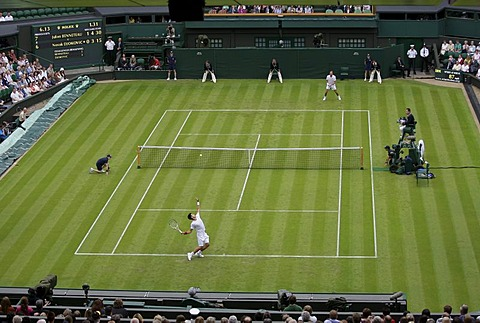
\includegraphics[width=0.4\textwidth]{img/tennis.jpg}}
        \qquad
        \subfloat{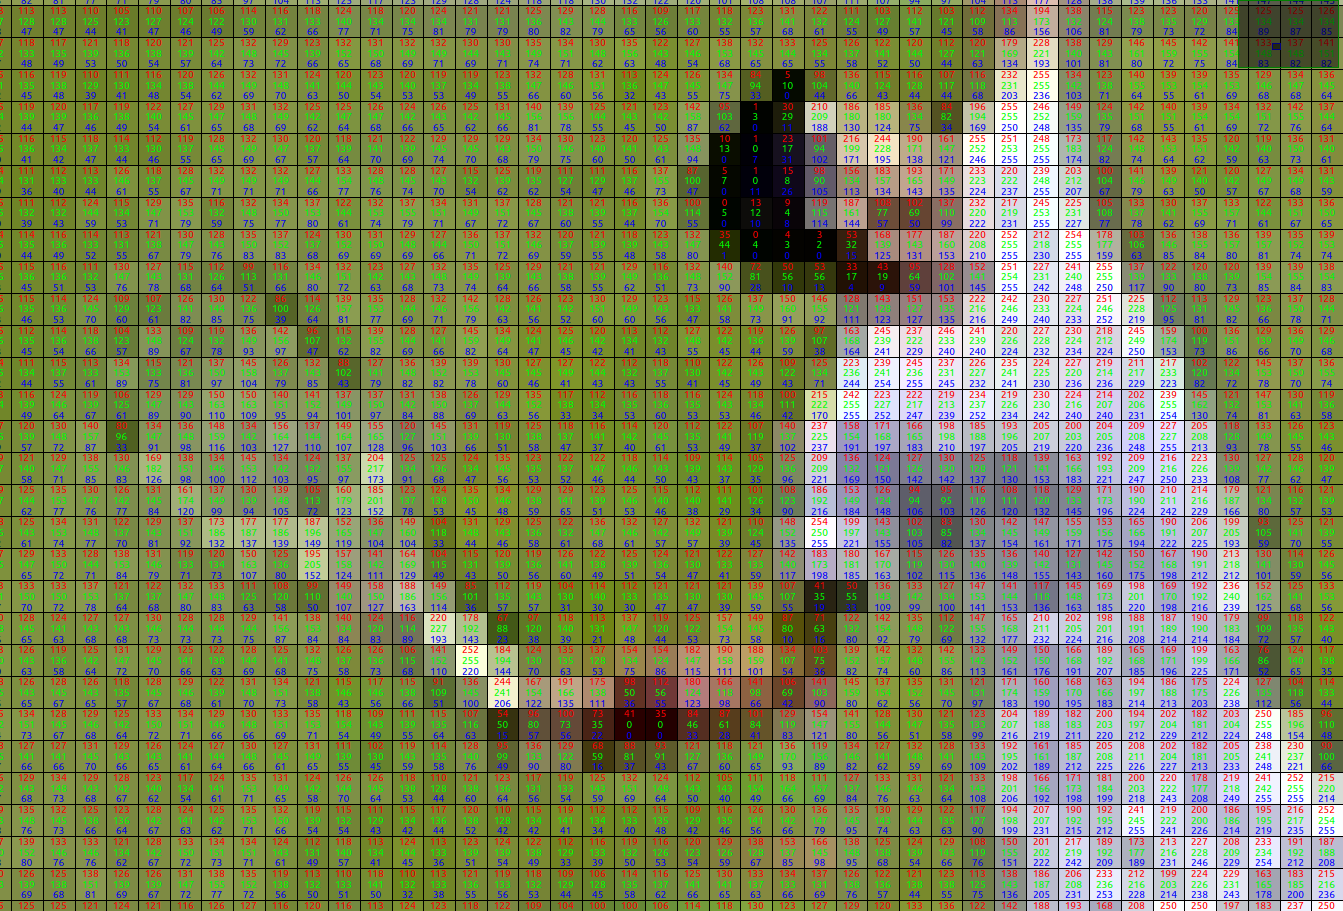
\includegraphics[width=0.4\textwidth]{img/pixels2.png}}
    \end{figure}
\end{frame}

